\section{Q9 — Spatial Correlation Variation by Stratum}\label{sec:strata}

We repeated the spatial analyses but now \emph{within strata} (UTC hour of day, season,
and year) to test whether coherence is stable across them. The answer is \textbf{yes for season and time of
day, but no for year}.

\subsection{Season: the strongest effect}

Coherence and decorrelation length both collapse in summer and peak in the transition seasons and
autumn (Figure~\ref{fig:seasondecay}): temperature $L$ falls from $\sim\SI{348}{km}$ (Fall) to
$\sim\SI{119}{km}$ (Summer), RH from $\sim\SI{284}{km}$ to $\sim\SI{88}{km}$, and V10 from
$\sim\SI{602}{km}$ to $\sim\SI{114}{km}$. This indicates that summer errors are more local, so they
decorrelate over much shorter distances. Pressure is the exception, remaining synoptic
(\,$L \approx \SI{443}{km}$) all year.

\begin{figure}[H]
  \centering
  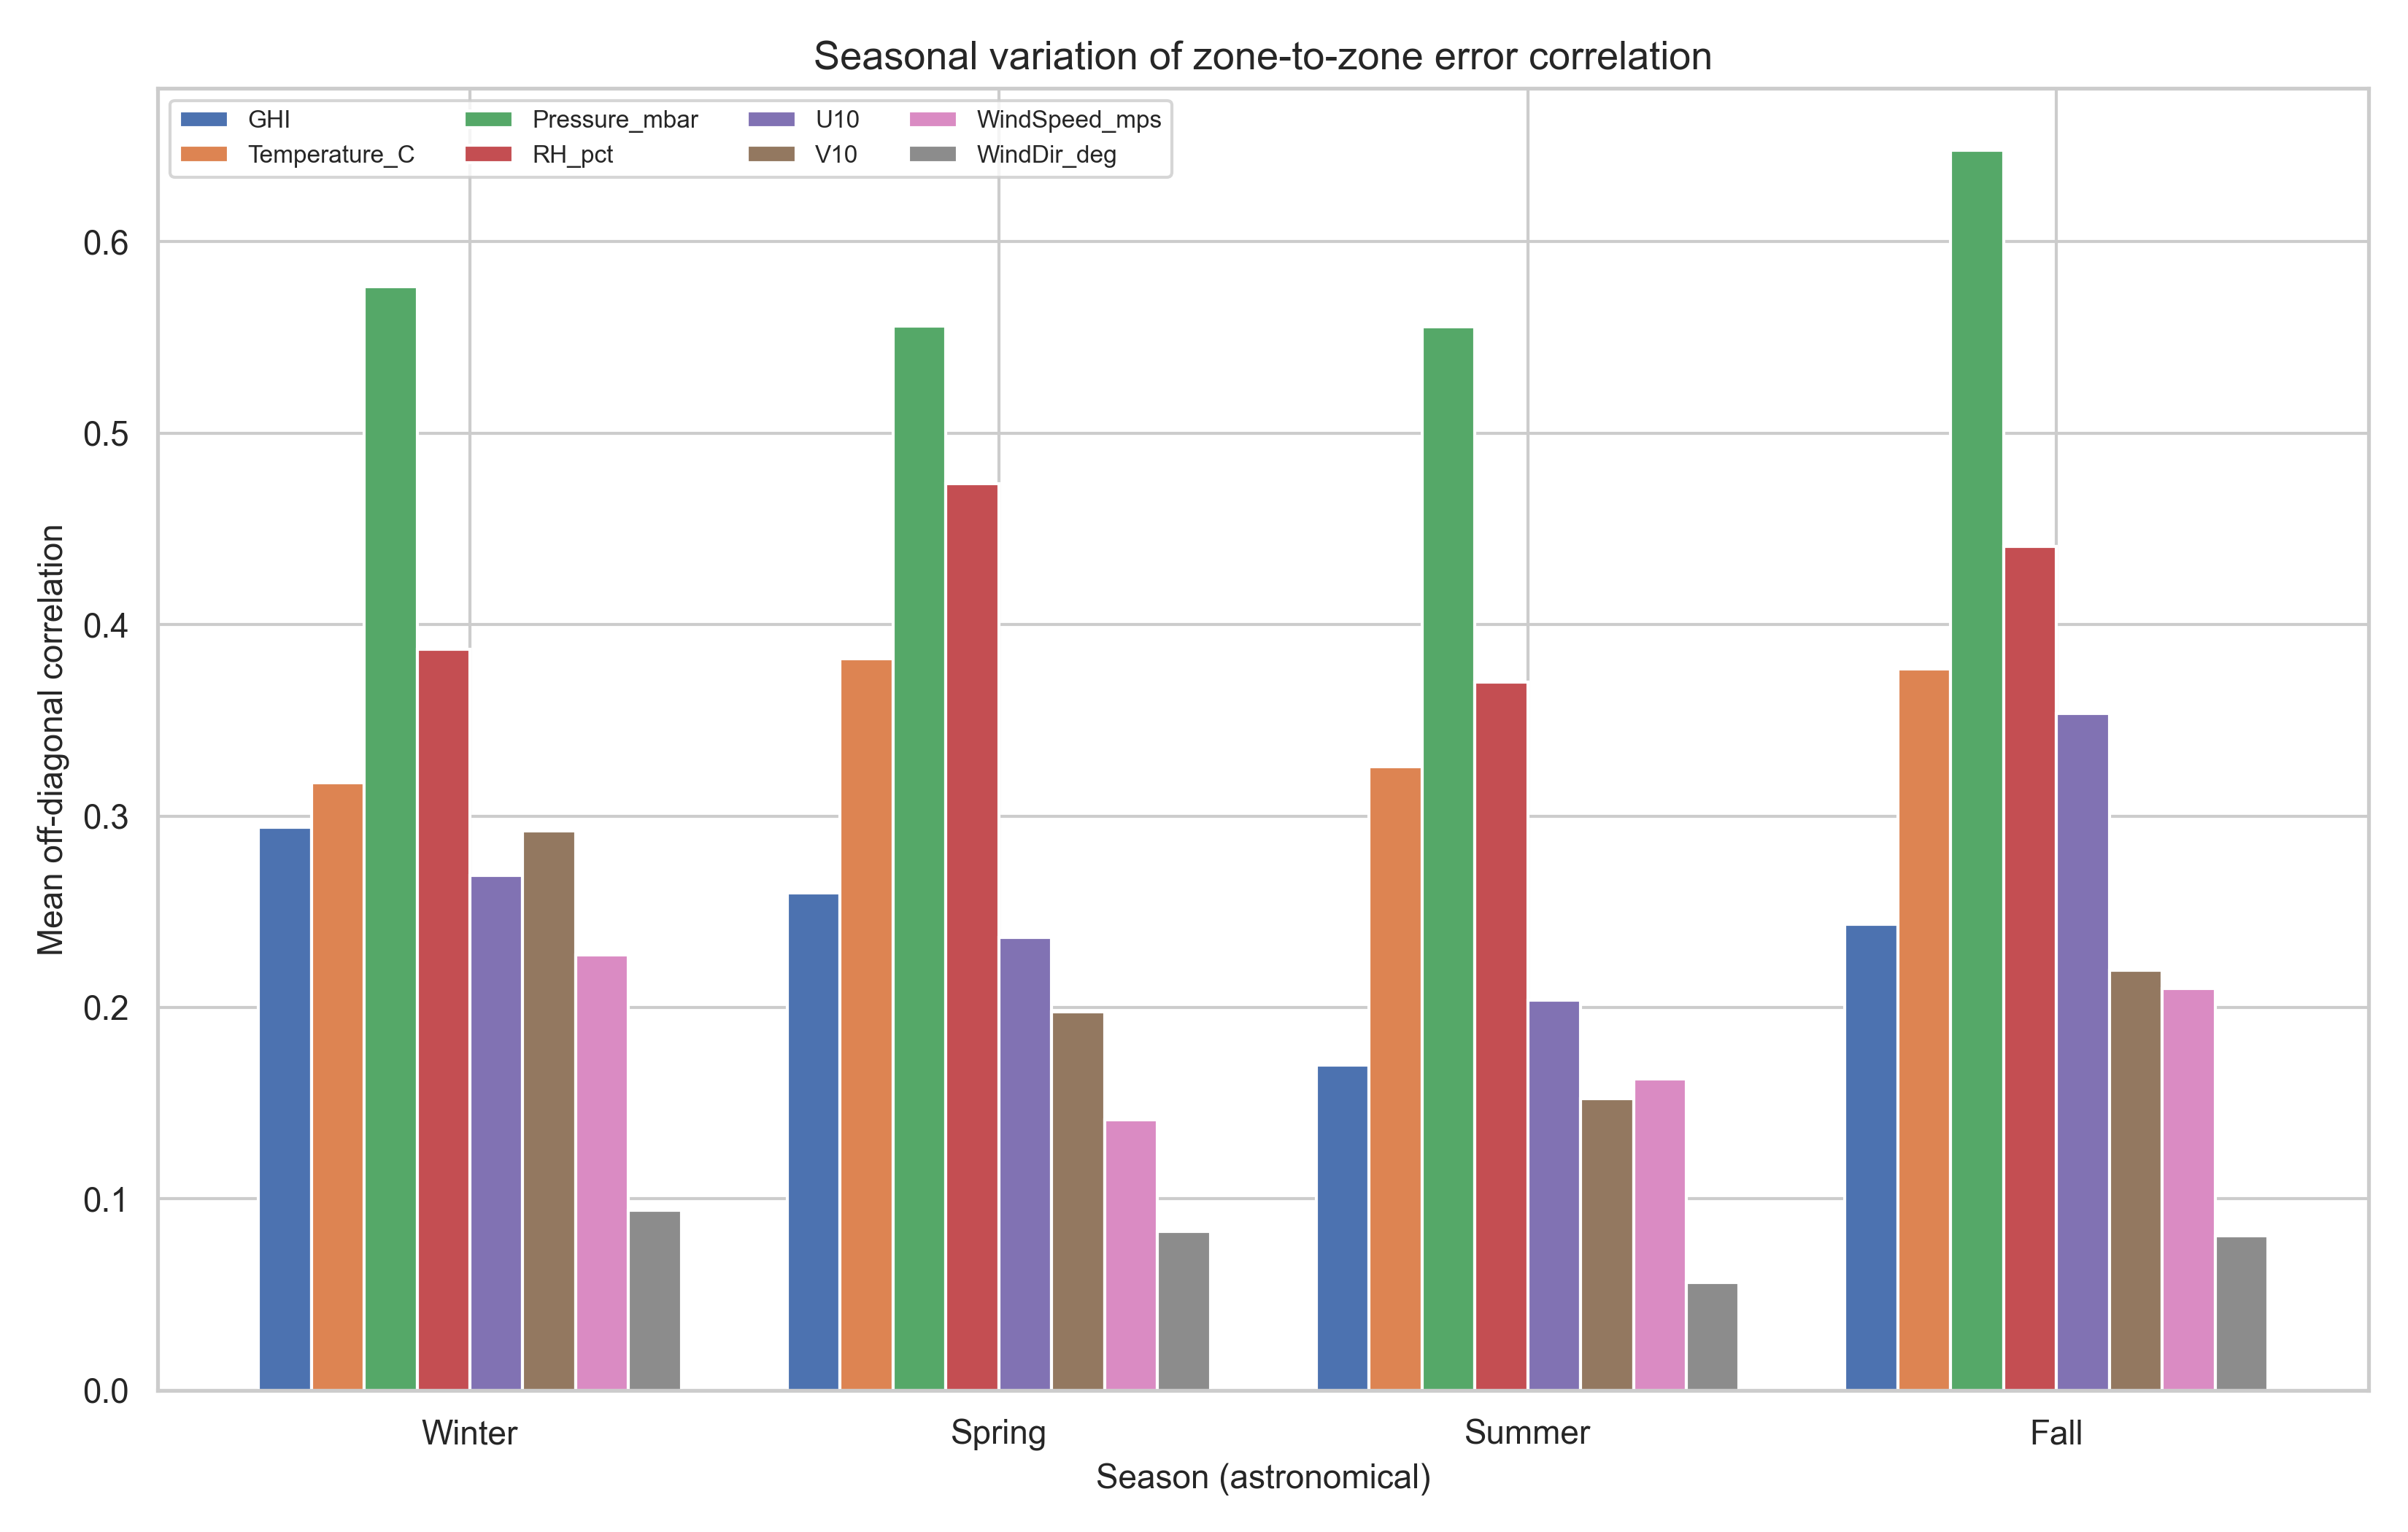
\includegraphics[width=\textwidth]{figures/Q9/seasonal_zone_correlation.png}
  \caption{Mean zone-to-zone correlation by season. Coherence is lowest in summer for every
  variable and highest in fall/winter; pressure and RH stay the most cross-zone coherent
  throughout. Summer is therefore the season in which neighbouring zones' errors are most
  independent.}
  \label{fig:seasoncorr}
\end{figure}

\begin{figure}[H]
  \centering
  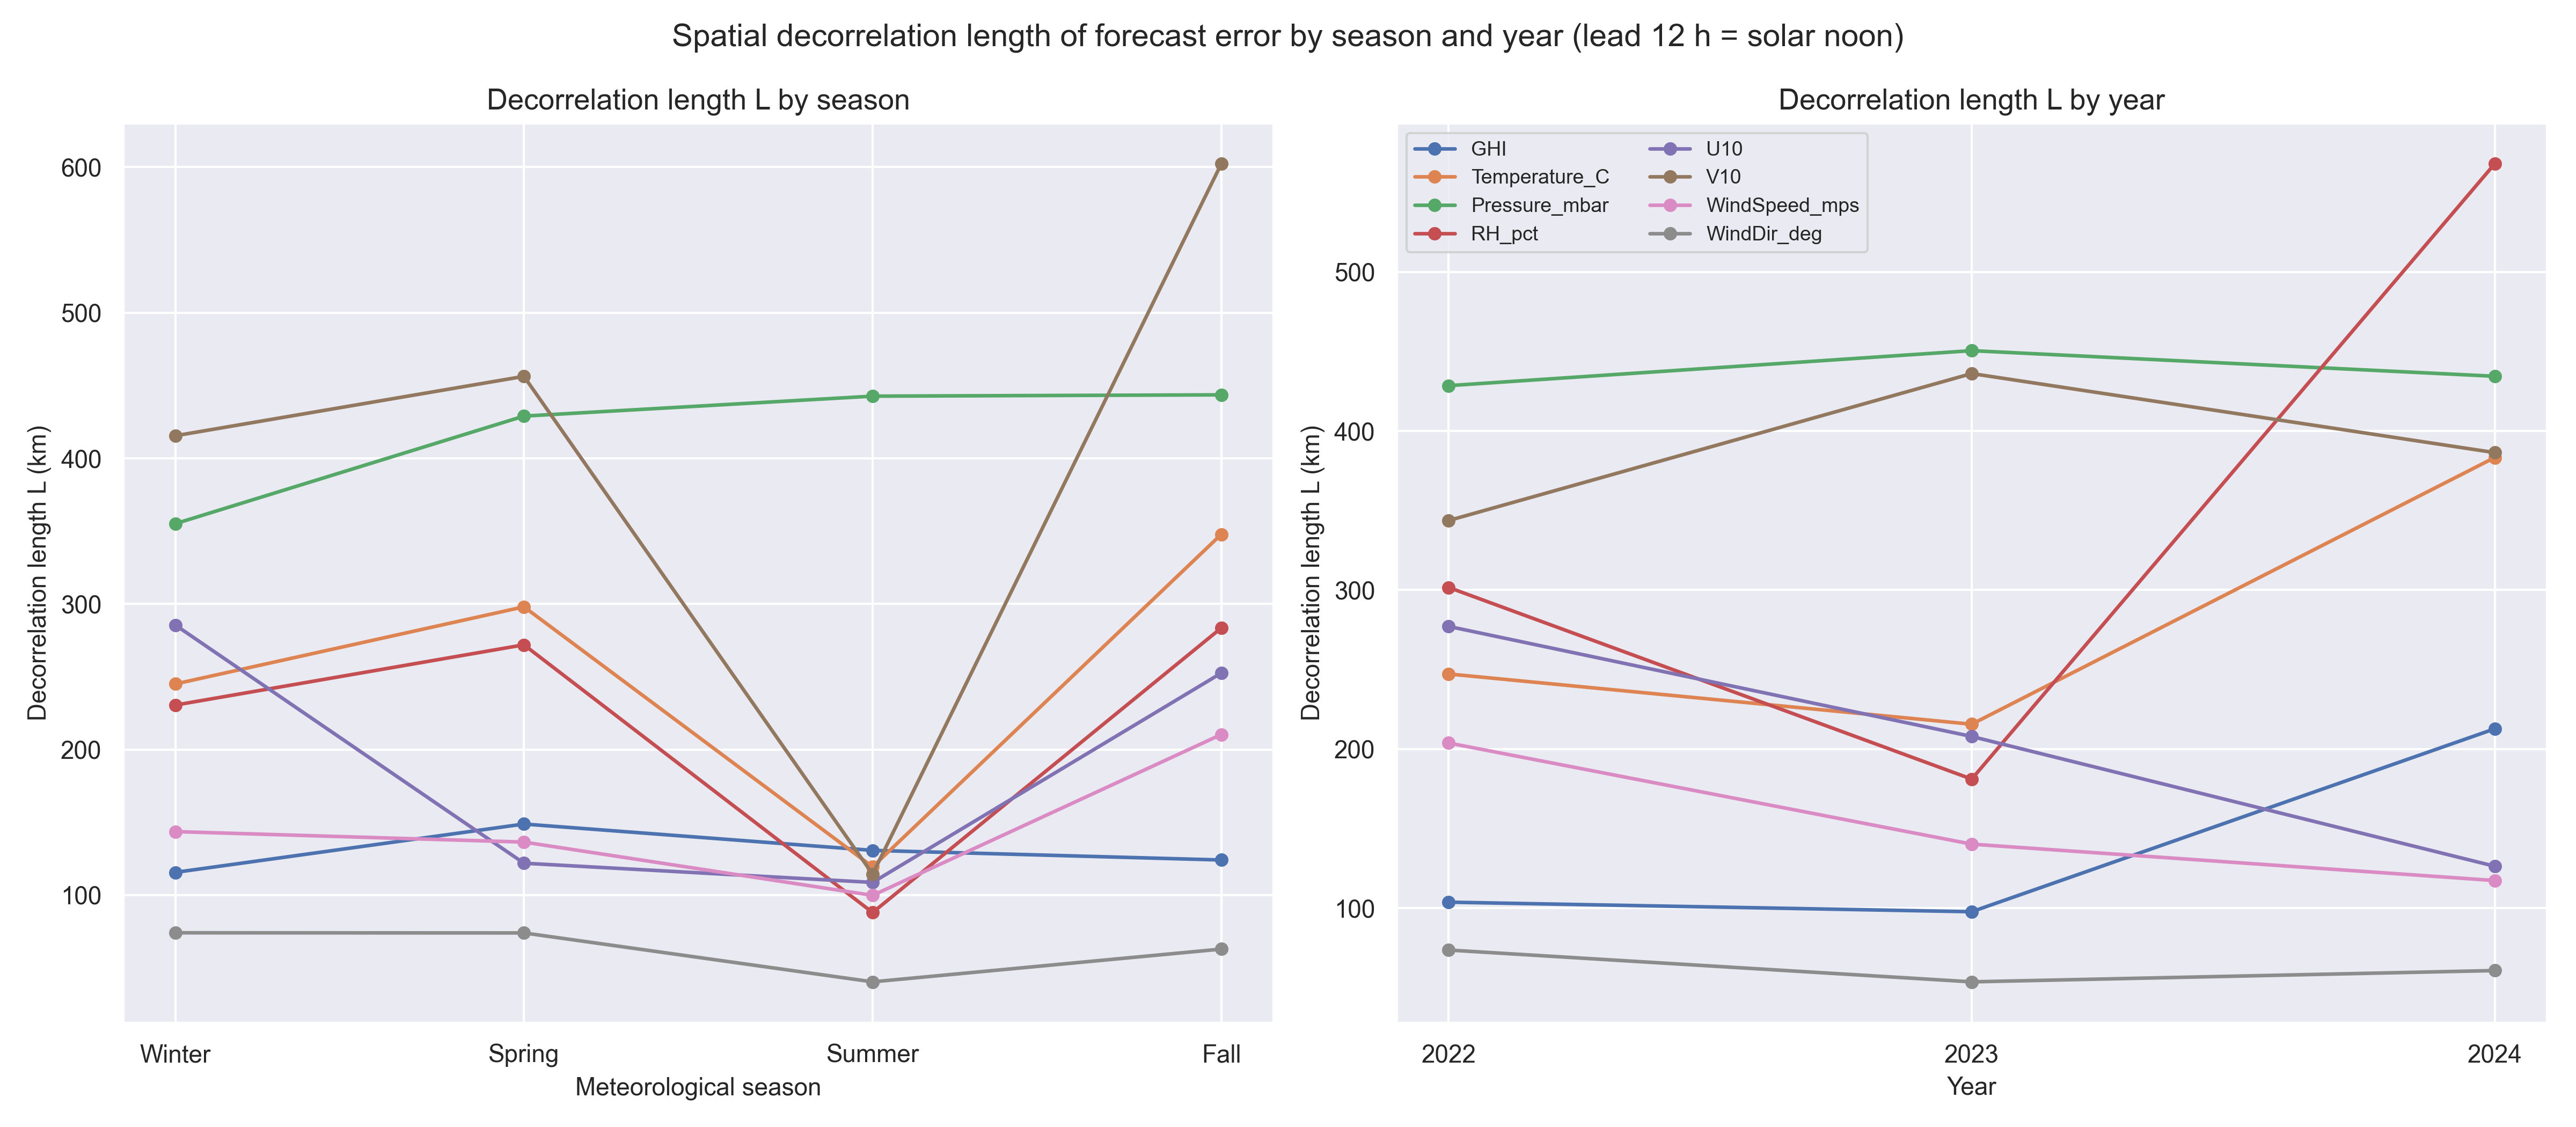
\includegraphics[width=\textwidth]{figures/Q9/decorrelation_length_by_season_year.png}
  \caption{Fitted decorrelation length $L$ by season (left) and year (right). $L$ collapses in
  summer as errors go local/convective, while pressure stays synoptic all year. The year panel is
  flat for pressure but swings 2--3$\times$ for RH/GHI/winds; a day-block bootstrap shows those
  year-to-year swings are within sampling uncertainty (see text).}
  \label{fig:seasondecay}
\end{figure}

\subsection{Time of day: a clear diurnal cycle}

Temperature and RH zone coherence dip in the mid-morning UTC hours
($\sim\!10\text{--}\SI{11}{}z$, the sunrise period) and rebound by late
afternoon ($\sim\!\SI{18}{}z$); pressure is flat across the day; GHI exists only in daytime UTC
hours and is modestly higher near solar noon; wind direction sits at a flat low floor
($\approx 0.08$). See Figure~\ref{fig:diurnal}.

\begin{figure}[H]
  \centering
  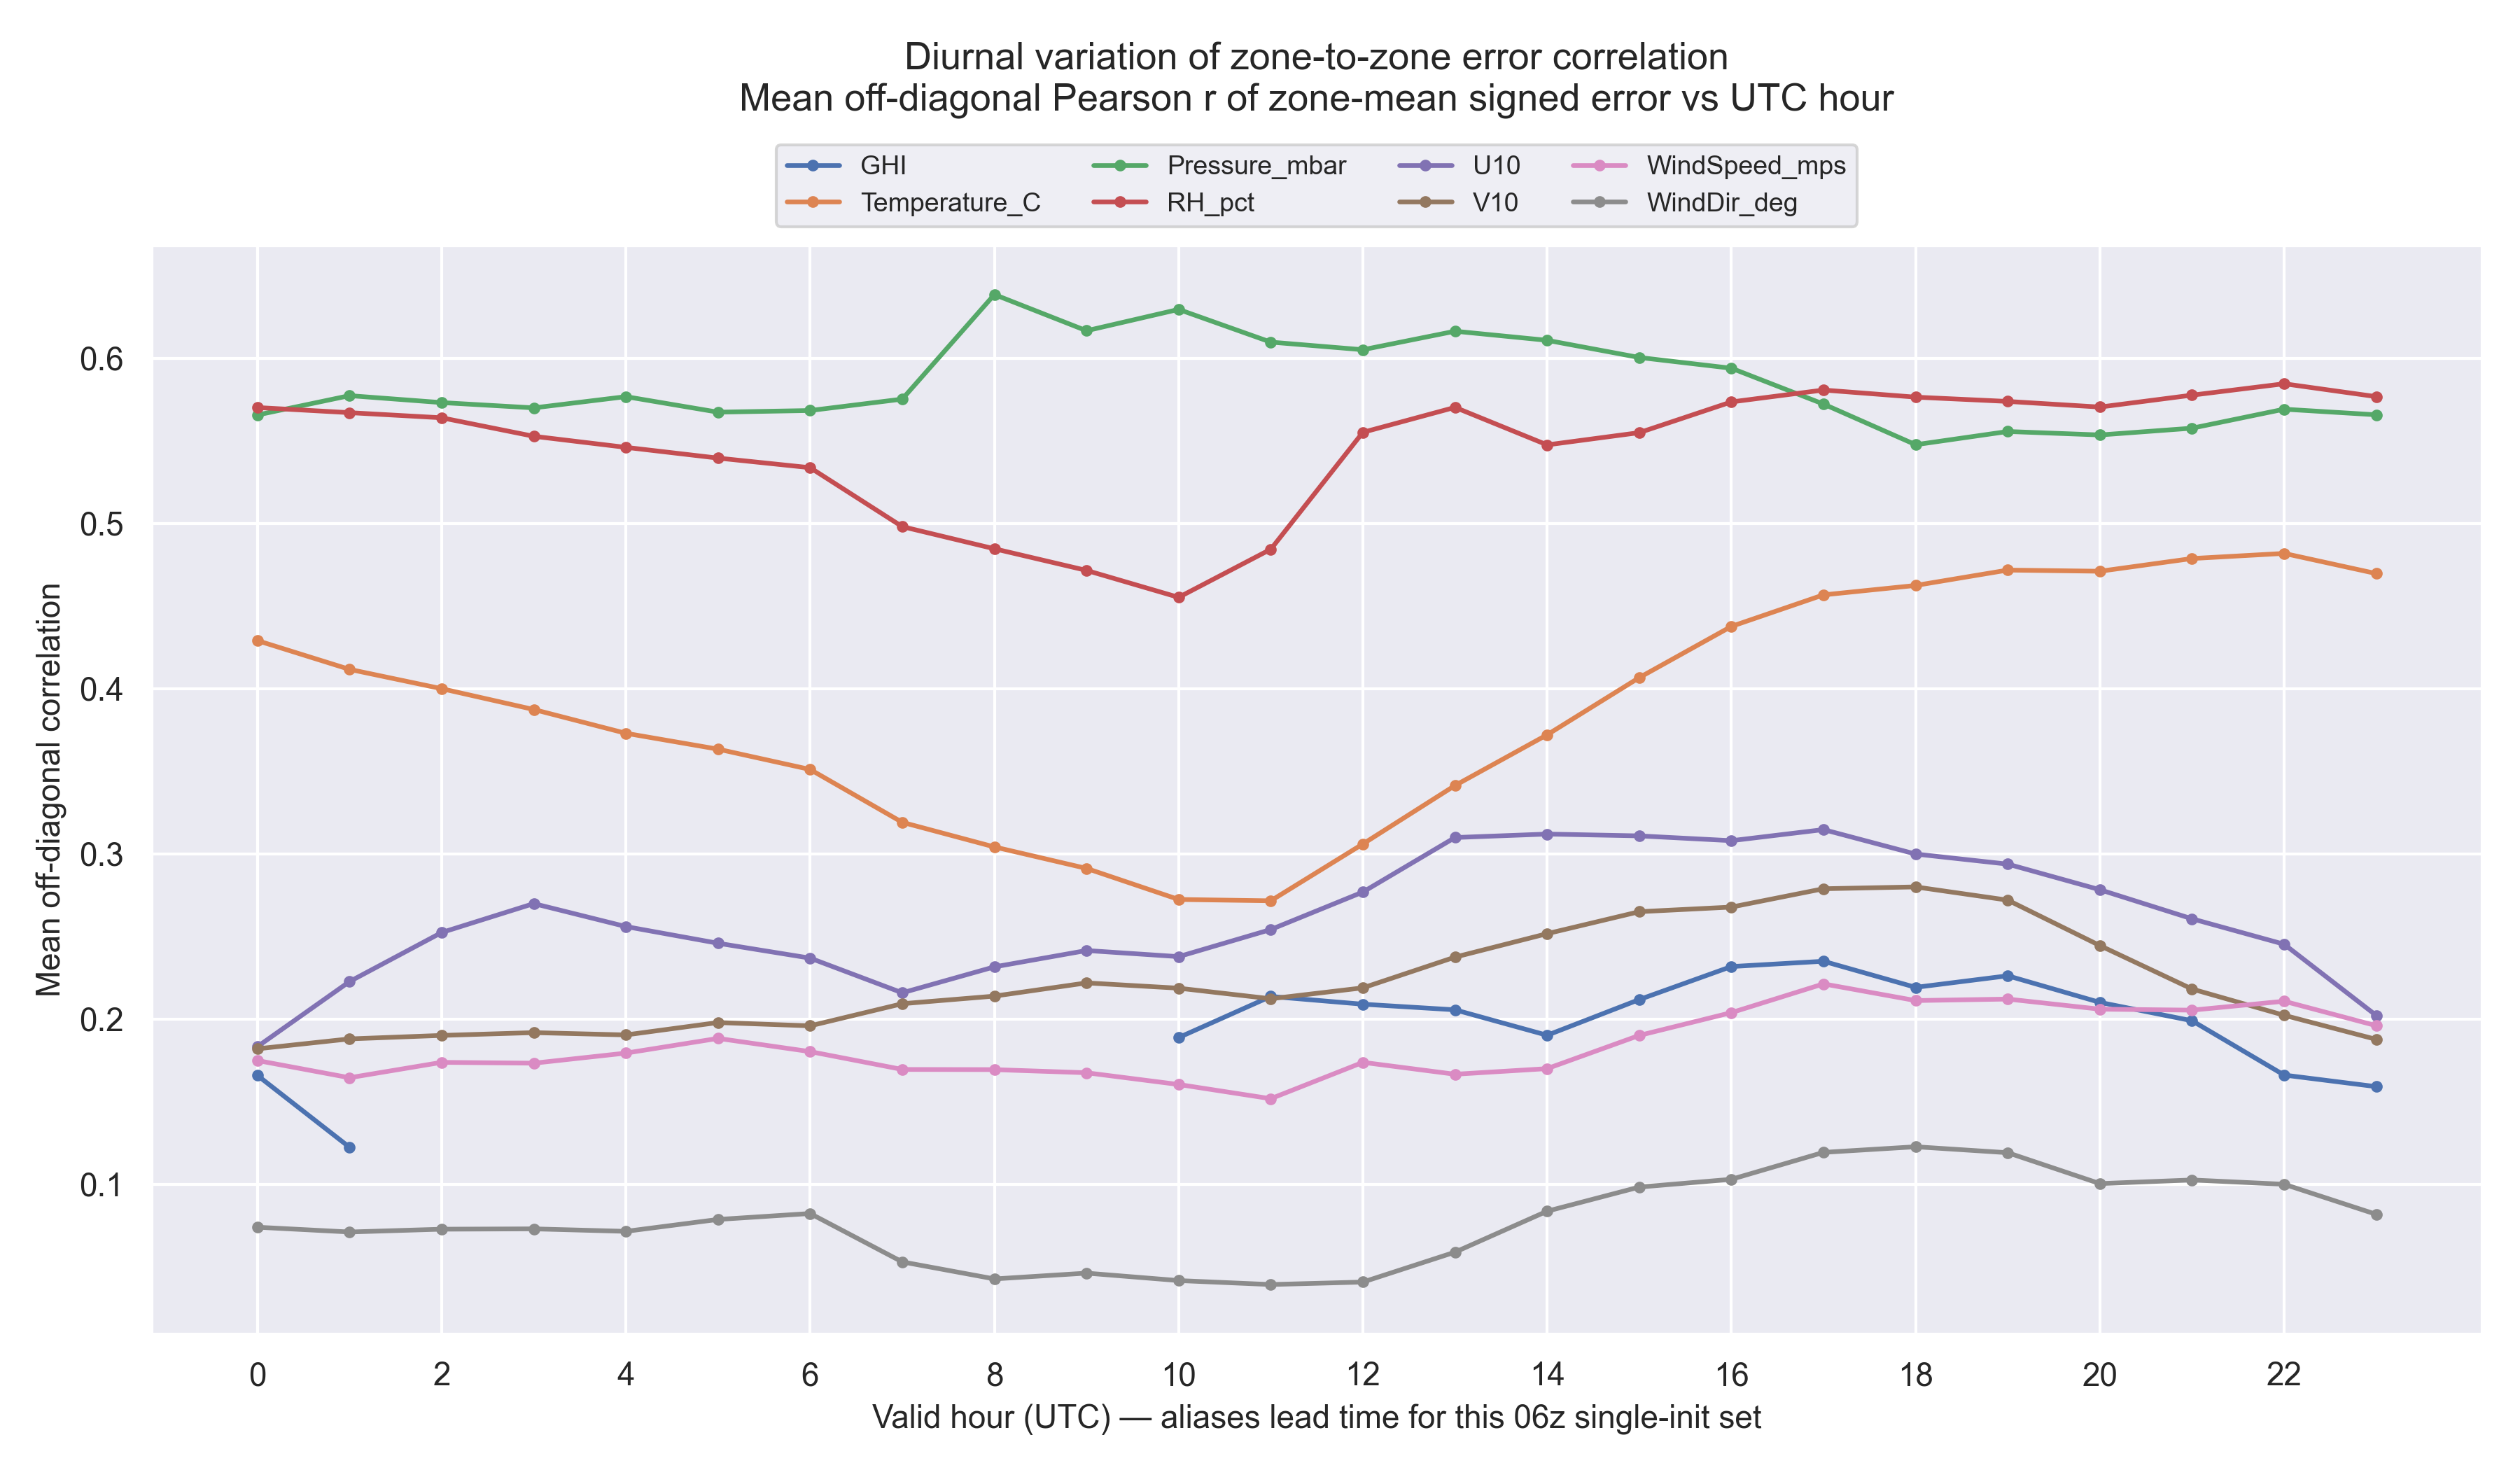
\includegraphics[width=\textwidth]{figures/Q9/diurnal_zone_correlation.png}
  \caption{Mean zone-to-zone correlation versus UTC hour. Temperature/RH coherence dips near
  sunrise (\,$\sim\!10\text{--}\SI{11}{}z$) and recovers by afternoon; pressure is flat; GHI is
  daytime-only and peaks near solar noon; wind direction is a flat low floor.}
  \label{fig:diurnal}
\end{figure}

\subsection{Year: stable, with a caveat on $L$}

The robust measures are flat across 2022--2024 (Figure~\ref{fig:yearcorr}): zone correlation moves only a few hundredths
(e.g.\ pressure $0.585 \to 0.571 \to 0.605$) and $d(r{=}0.5)$ is steady for clean-decay variables
, e.g. pressure $\sim\!294\text{--}\SI{304}{km}$. Although the \emph{fitted} $L$ swings 2--3$\times$ for the weakly-coherent variables (RH $302\to181\to\SI{568}{km}$; GHI $104\to98\to\SI{213}{km}$), a
day-block bootstrap shows the within-year sampling uncertainty is as large as those gaps. Hence, the
dramatic 2024 spikes across several variables sit only $\sim$1--1.6$\sigma$ above the other years and are not
significant. \textbf{Therefore, year-to-year changes in $L$ should not be read as real change between years}.

\begin{figure}[H]
  \centering
  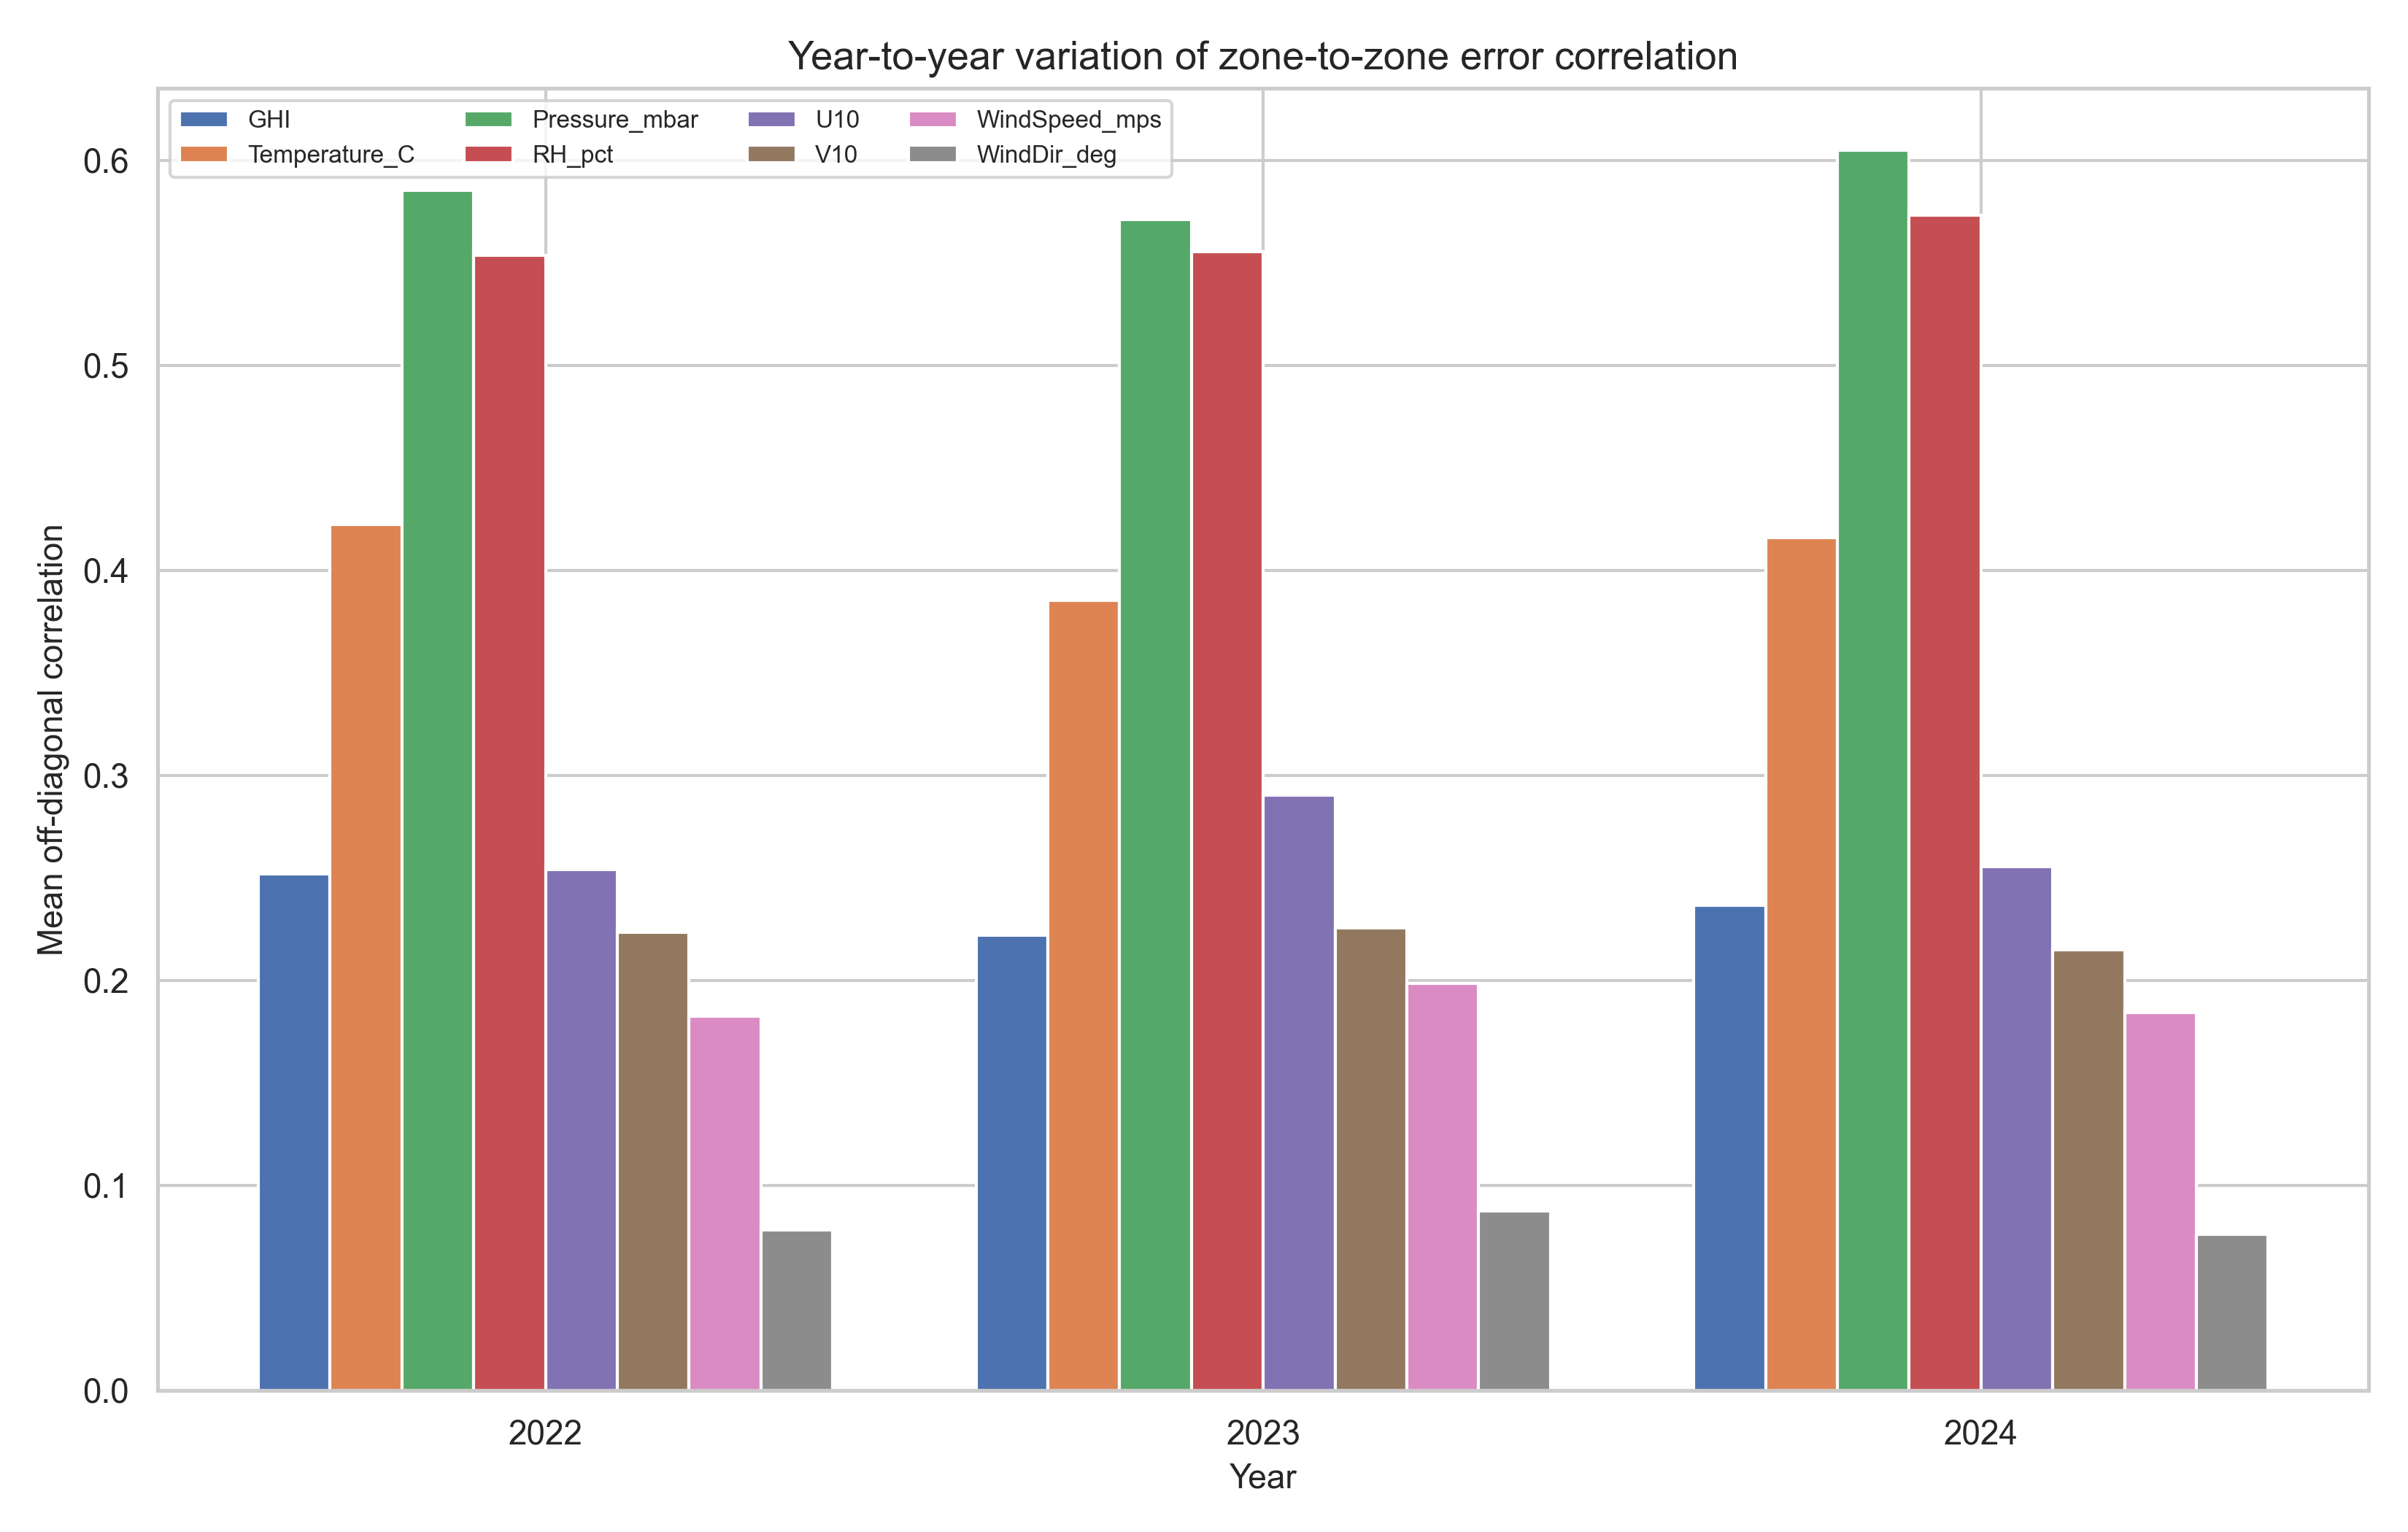
\includegraphics[width=\textwidth]{figures/Q9/yearly_zone_correlation.png}
  \caption{Year-to-year variation of zone-to-zone forecast-error correlation. Each bar is the
  mean off-diagonal Pearson~$r$ of the $9\times 9$ zone-to-zone correlation matrix (zone-mean
  signed error, all lead times pooled) for one variable in one year. The bars are nearly
  identical across 2022, 2023, and 2024---pressure and RH stay the most cross-zone coherent
  ($r\approx0.55$--$0.61$), temperature is intermediate ($\approx0.4$), GHI and the wind
  components sit near $0.2$--$0.3$, and wind direction is a flat low floor ($\approx0.08$)---so
  the spatial-correlation structure of the error is essentially stable from year to year. Models
  or portfolio strategies calibrated on one year therefore carry over to the next. (GHI uses
  daytime samples only, $\text{GHI}_{\text{act}}>\SI{5}{W/m^2}$.)}
  \label{fig:yearcorr}
\end{figure}

\subsection{Portfolio takeaway}

Cross-zone error diversification is best in \textbf{summer} (shortest decorrelation lengths,
lowest GHI coherence), weakest in autumn/winter, and stable from year to year. Pressure error
never diversifies away in any stratum.
